% Options for packages loaded elsewhere
\PassOptionsToPackage{unicode}{hyperref}
\PassOptionsToPackage{hyphens}{url}
%
\documentclass[
]{article}
\usepackage{lmodern}
\usepackage{amsmath}
\usepackage{ifxetex,ifluatex}
\ifnum 0\ifxetex 1\fi\ifluatex 1\fi=0 % if pdftex
  \usepackage[T1]{fontenc}
  \usepackage[utf8]{inputenc}
  \usepackage{textcomp} % provide euro and other symbols
  \usepackage{amssymb}
\else % if luatex or xetex
  \usepackage{unicode-math}
  \defaultfontfeatures{Scale=MatchLowercase}
  \defaultfontfeatures[\rmfamily]{Ligatures=TeX,Scale=1}
\fi
% Use upquote if available, for straight quotes in verbatim environments
\IfFileExists{upquote.sty}{\usepackage{upquote}}{}
\IfFileExists{microtype.sty}{% use microtype if available
  \usepackage[]{microtype}
  \UseMicrotypeSet[protrusion]{basicmath} % disable protrusion for tt fonts
}{}
\makeatletter
\@ifundefined{KOMAClassName}{% if non-KOMA class
  \IfFileExists{parskip.sty}{%
    \usepackage{parskip}
  }{% else
    \setlength{\parindent}{0pt}
    \setlength{\parskip}{6pt plus 2pt minus 1pt}}
}{% if KOMA class
  \KOMAoptions{parskip=half}}
\makeatother
\usepackage{xcolor}
\IfFileExists{xurl.sty}{\usepackage{xurl}}{} % add URL line breaks if available
\IfFileExists{bookmark.sty}{\usepackage{bookmark}}{\usepackage{hyperref}}
\hypersetup{
  pdftitle={The Impact of Chocolate on Graduate Student Happiness},
  pdfauthor={Sam Harper, McGill University},
  hidelinks,
  pdfcreator={LaTeX via pandoc}}
\urlstyle{same} % disable monospaced font for URLs
\usepackage[margin=1in]{geometry}
\usepackage{graphicx}
\makeatletter
\def\maxwidth{\ifdim\Gin@nat@width>\linewidth\linewidth\else\Gin@nat@width\fi}
\def\maxheight{\ifdim\Gin@nat@height>\textheight\textheight\else\Gin@nat@height\fi}
\makeatother
% Scale images if necessary, so that they will not overflow the page
% margins by default, and it is still possible to overwrite the defaults
% using explicit options in \includegraphics[width, height, ...]{}
\setkeys{Gin}{width=\maxwidth,height=\maxheight,keepaspectratio}
% Set default figure placement to htbp
\makeatletter
\def\fps@figure{htbp}
\makeatother
\setlength{\emergencystretch}{3em} % prevent overfull lines
\providecommand{\tightlist}{%
  \setlength{\itemsep}{0pt}\setlength{\parskip}{0pt}}
\setcounter{secnumdepth}{-\maxdimen} % remove section numbering
\usepackage{booktabs}
\usepackage{longtable}
\usepackage{array}
\usepackage{multirow}
\usepackage{wrapfig}
\usepackage{float}
\usepackage{colortbl}
\usepackage{pdflscape}
\usepackage{tabu}
\usepackage{threeparttable}
\usepackage{threeparttablex}
\usepackage[normalem]{ulem}
\usepackage{makecell}
\usepackage{xcolor}
\ifluatex
  \usepackage{selnolig}  % disable illegal ligatures
\fi
\newlength{\cslhangindent}
\setlength{\cslhangindent}{1.5em}
\newlength{\csllabelwidth}
\setlength{\csllabelwidth}{3em}
\newenvironment{CSLReferences}[3] % #1 hanging-ident, #2 entry spacing
 {% don't indent paragraphs
  \setlength{\parindent}{0pt}
  % turn on hanging indent if param 1 is 1
  \ifodd #1 \everypar{\setlength{\hangindent}{\cslhangindent}}\ignorespaces\fi
  % set entry spacing
  \ifnum #2 > 0
  \setlength{\parskip}{#2\baselineskip}
  \fi
 }%
 {}
\usepackage{calc} % for \widthof, \maxof
\newcommand{\CSLBlock}[1]{#1\hfill\break}
\newcommand{\CSLLeftMargin}[1]{\parbox[t]{\maxof{\widthof{#1}}{\csllabelwidth}}{#1}}
\newcommand{\CSLRightInline}[1]{\parbox[t]{\linewidth}{#1}}
\newcommand{\CSLIndent}[1]{\hspace{\cslhangindent}#1}

\title{The Impact of Chocolate on Graduate Student Happiness}
\author{Sam Harper, McGill University}
\date{2020-10-30}

\begin{document}
\maketitle

\hypertarget{abstract}{%
\subsection{Abstract}\label{abstract}}

\begin{itemize}
\tightlist
\item
  Why did we start? Because chocolate.
\item
  What did we do? Ate chocolate.
\item
  What did we find? It's delicious.
\item
  What does it all matter? It's obvious!
\end{itemize}

\hypertarget{background}{%
\subsection{Background}\label{background}}

Let's face it. Chocolate is delicious, and it seems impossible that it
might not be good for you. However, the science is unclear, at least for
some outcomes.(Chan 2007)

\hypertarget{methods}{%
\subsection{Methods}\label{methods}}

We recruited students who thought they were coming for training in
reproducible research methods as a pre-text for eating chocolate in the
morning. We measured their happiness using our established, validated
index.

We calculated some descriptive statistics and ran a simple linear
regression model:

\[
y_{it}=\beta_{0} + \beta_{1}*Treated + \beta_{2}*Period + \epsilon_{it}
\]

We also explored a model with a product term, but not because
p\textgreater0.05 in the previous model. Honest.

\hypertarget{results}{%
\subsection{Results}\label{results}}

Descriptive statistics are shown in Table 1

\begin{table}

\caption{\label{tab:table1}Mean happiness by treatment and time}
\centering
\begin{tabular}[t]{llrr}
\toprule
Period & Treatment & Mean & SD\\
\midrule
 & Control & 9.89 & 8.15\\
\cmidrule{2-4}
\multirow{-2}{*}{\raggedright\arraybackslash Pre} & Treated & 9.78 & 6.91\\
\cmidrule{1-4}
 & Control & 14.83 & 6.95\\
\cmidrule{2-4}
\multirow{-2}{*}{\raggedright\arraybackslash Intervention} & Treated & 17.70 & 7.36\\
\cmidrule{1-4}
 & Control & 20.21 & 7.03\\
\cmidrule{2-4}
\multirow{-2}{*}{\raggedright\arraybackslash Post} & Treated & 25.30 & 7.26\\
\bottomrule
\end{tabular}
\end{table}

Estimates from the regression analysis are shown in Table 2. Regression
results clearly show that chocolate increases happiness. We can see that
the overall happiness index for the chocolate group was 4.67 units
higher in the post period relative to the change over the same period in
the control group {[}95\% CI: 3.66, 5.68{]}.

\begin{table}[!htbp] \centering 
  \caption{Effect of chocolate on happiness} 
  \label{} 
\begin{tabular}{@{\extracolsep{5pt}}lcc} 
\\[-1.8ex]\hline 
\hline \\[-1.8ex] 
 & Adjusted model & Interaction Model \\ 
 Treated: Yes & 2.62 & $-$0.11 \\ 
  & (1.88, 3.37) & ($-$1.39, 1.17) \\ 
  & & \\ 
 Time: Intervention & 6.43 & 4.94 \\ 
  & (5.52, 7.35) & (3.66, 6.22) \\ 
  & & \\ 
 Time: Post & 12.92 & 10.32 \\ 
  & (12.01, 13.83) & (9.04, 11.59) \\ 
  & & \\ 
 Treated x Intervention &  & 2.99 \\ 
  &  & (1.18, 4.79) \\ 
  & & \\ 
 Treated x Post &  & 5.21 \\ 
  &  & (3.40, 7.01) \\ 
  & & \\ 
 Constant & 8.52 & 9.89 \\ 
  & (7.78, 9.27) & (8.98, 10.79) \\ 
  & & \\ 
\hline \\[-1.8ex] 
\hline 
\hline \\[-1.8ex] 
\end{tabular} 
\end{table}

Regression results clearly show that chocolate increases happiness, but
if you aren't convinced please see Figure 1.

\begin{figure}
\centering
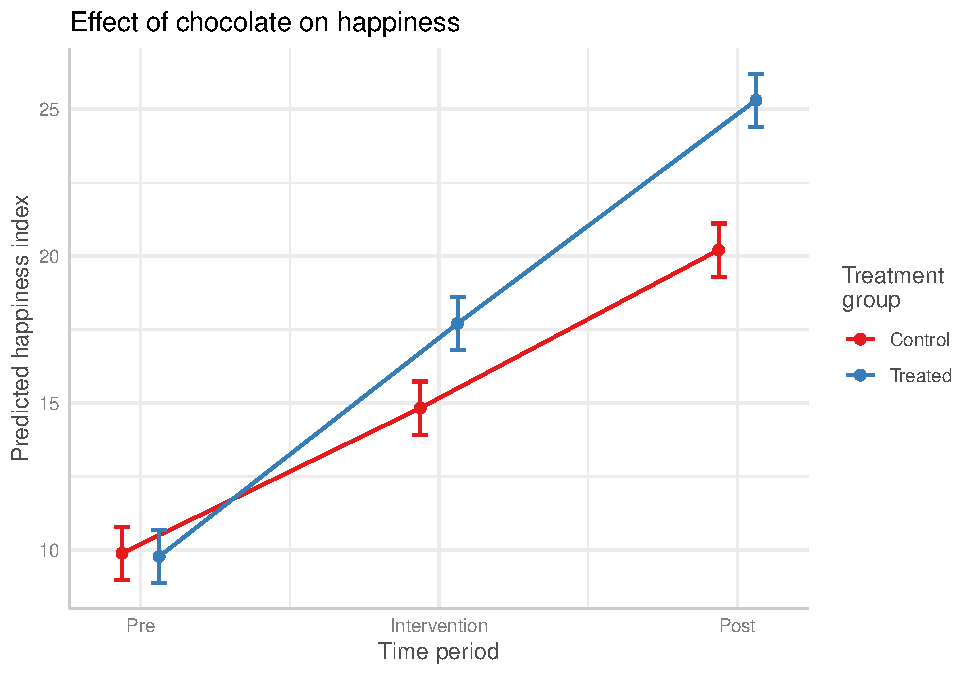
\includegraphics{choc-paper-rmd_files/figure-latex/figure1-1.pdf}
\caption{Predicted happiness index from interaction model}
\end{figure}

\hypertarget{discussion}{%
\subsection{Discussion}\label{discussion}}

We think this is convincing. But it may not matter for policy since
another randomized trial showed that many participants switched groups
mid-study because of their personal chocolate preferences.(Scaramuzza
and Zuccotti 2015)

\hypertarget{references}{%
\subsection*{References}\label{references}}
\addcontentsline{toc}{subsection}{References}

\hypertarget{refs}{}
\begin{CSLReferences}{1}{0}
\leavevmode\hypertarget{ref-Chan:2007th}{}%
Chan, Kevin. 2007. {``A Clinical Trial Gone Awry: The {Chocolate
Happiness Undergoing More Pleasantness (CHUMP)} Study.''} \emph{CMAJ}
177 (12): 1539--41. \url{https://doi.org/10.1503/cmaj.071161}.

\leavevmode\hypertarget{ref-Scaramuzza:2015fy}{}%
Scaramuzza, Andrea E, and Gian Vincenzo Zuccotti. 2015. {``Dark
Chocolate Consumption and Lower {HbA1c} in Children with Diabetes:
Direct Cause or Pure Happiness?''} \emph{Clin Nutr} 34 (2): 333--34.
\url{https://doi.org/10.1016/j.clnu.2015.01.007}.

\end{CSLReferences}

\end{document}
